% preamble ---------------------------------------------------------------
\documentclass[xcolor=dvipsnames]{beamer}

% meta data --------------------------------------------------------------
\title[Text supporting CV models]{Seminar: Multimodal Deep Learning}
\subtitle{Topic 7: Text supporting CV models}
\author[Max Schneider]{Author: Maximilian Schneider\\
        Supervisor: Jann Goschenhofer}
\institute[]{Department Of Statistics\\
             Ludwig-Maximilians-Universität\\
             \vspace{0.5cm}
             
\includegraphics[scale=0.02]{../../figures/Sigillum}%
            }
\date{\today}

% theme
\usetheme{Madrid}
\usecolortheme{dove}
\beamertemplatenavigationsymbolsempty  % no navigation symbols
\setbeamertemplate{section in toc}{\hspace*{1em}\textcolor{OliveGreen}{\inserttocsectionnumber}~\inserttocsection\par}
\setbeamertemplate{subsection in toc}{\hspace*{2em}\textcolor{OliveGreen}{\inserttocsectionnumber.\inserttocsubsectionnumber}~\inserttocsubsection\par}  % numbered table of contents
\setbeamercovered{transparent}
\usefonttheme[onlymath]{serif}  % better math font
\setbeamertemplate{caption}[numbered]

% packages ---------------------------------------------------------------
% text encoding
\usepackage[utf8]{inputenc}

% better interaction with pdf (strg + f)
\usepackage[T1]{fontenc}

% comment, quote environment (load csquotes before babel)
\usepackage{comment, csquotes}

% language, line breaks
\usepackage[english]{babel}

% date format
\usepackage[datesep=.]{datetime2}
\DTMsetdatestyle{ddmmyyyy}

% bibliography
\usepackage[style=authoryear, backend=biber, sorting=nty, uniquename=false]{biblatex}
\addbibresource{../../book.bib}
\renewcommand*{\bibsetup}{%
  \interlinepenalty=10000\relax % default is 5000
  \widowpenalty=10000\relax
  \clubpenalty=10000\relax
  \raggedbottom
  \frenchspacing
  \biburlsetup}

% load external figures, embed functioning links
\usepackage{graphicx, hyperref}

% sub-figures
\usepackage{caption, subcaption}

% one table cell over multiple columns
\usepackage{multicol}

% rotate long table headers
\usepackage{booktabs}
\newcommand*\rot{\rotatebox{90}}

% math symbols
\usepackage{amsmath, amssymb, bm}

\begin{document} %--------------------------------------------------------

{
\setbeamertemplate{footline}{}
\begin{frame}
  \titlepage
\end{frame}
}
\addtocounter{framenumber}{-1}

\section{Introduction} %--------------------------------------------------

\begin{frame}{Introduction: Scale}
  \blockquote{
    The biggest lesson that can be read from 70 years of AI research is that general methods that leverage computation are ultimately the most effective, and by a large margin.
    \ldots
    Most AI research has been conducted as if the computation available to the agent were constant (in which case leveraging human knowledge would be one of the only ways to improve performance) but, over a slightly longer time than a typical research project, massively more computation inevitably becomes available.
    Seeking an improvement that makes a difference in the shorter term, researchers seek to leverage their human knowledge of the domain, but the only thing that matters in the long run is the leveraging of computation.
    \ldots
  }
\end{frame}

\begin{frame}{Introduction: Scale}
  \blockquote[\cite{sutton2019bitterlesson}]{
    \ldots
    One thing that should be learned from the bitter lesson is the great power of general purpose methods, of methods that continue to scale with increased computation even as the available computation becomes very great.
    The two methods that seem to scale arbitrarily in this way are search and learning.
  }
\end{frame}

\section{Concepts} %------------------------------------------------------
\begin{frame}{Contents}
  \tableofcontents[sections={1-2}, currentsection]
  \tableofcontents[sections={3-6}]
\end{frame}

\subsection{Web-scale data} %---------------------------------------------
\begin{frame}{Concepts: Web-scale data}
  \begin{itemize}
    \item Internet full of naturally occurring image-text pairs
    \item No labor intensive manual labeling
    \item Large datasets
      \begin{itemize}
        \item 400 million \parencite[CLIP;][]{radford2021learning}
        \item 900 million \parencite[Florence;][]{yuan2021florence}
        \item 1.8 billion \parencite[ALIGN;][]{jia2021scaling}
      \end{itemize}
    \item Pre-processing needed, resulting in arbitrary choices
    \item Social biases are reproduced
  \end{itemize}
\end{frame}

\subsection{Contrastive objective} %--------------------------------------
\begin{frame}{Concepts: Contrastive objective}
  \begin{equation}
    \ell_1^{V1, V2} = - \underset{\{v_1^1, v_2^1, \ldots, v_2^N\}}{\mathbb{E}} \left( \log \frac{h_\theta(\{v_1^1,v_2^1\})}{h_\theta(\{v_1^1,v_2^1\}) + \sum_{k=2}^N h_\theta(\{v_1^1, v_2^k\})} \right)
  \end{equation}

  \vspace{1cm}

  \begin{figure}[ht]
    \begin{minipage}{0.67\textwidth}
      \centering
      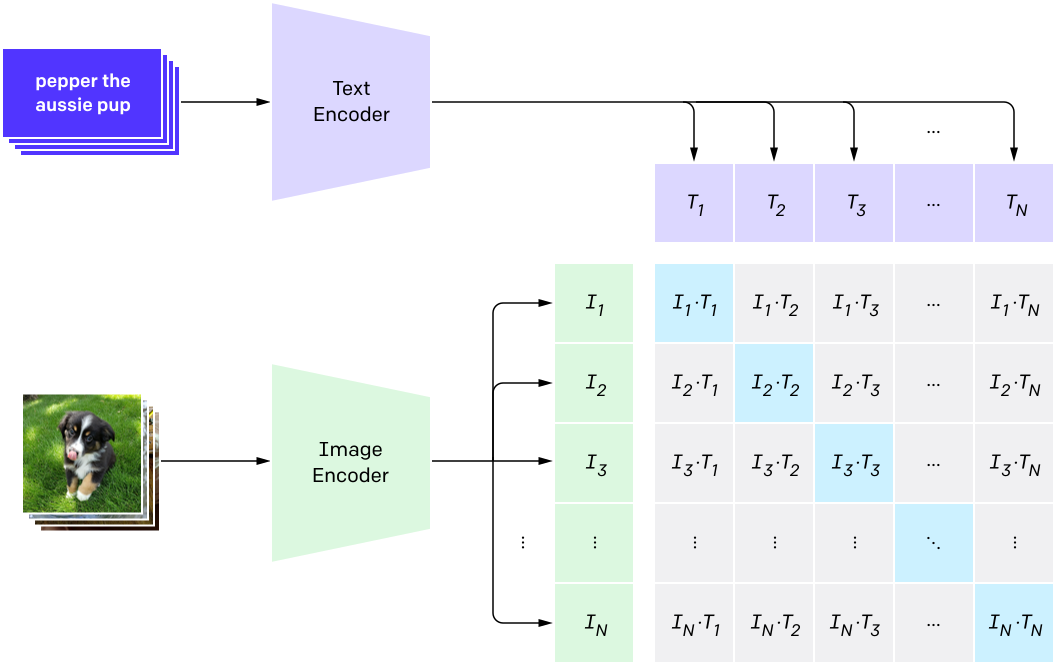
\includegraphics[width=0.9\linewidth]{../../figures/02-04-text-support-img/contrastive-pre-training}
    \end{minipage}
    \begin{minipage}[c]{0.3\textwidth}
      \caption{Visualization of contrastive objective \parencite{openai2021clipblog}}
    \end{minipage}
  \end{figure}
\end{frame}

\begin{frame}{Concepts: Contrastive objective}
  \begin{columns}
    \begin{column}{0.5\textwidth}
      \begin{figure}[ht]
        \centering
        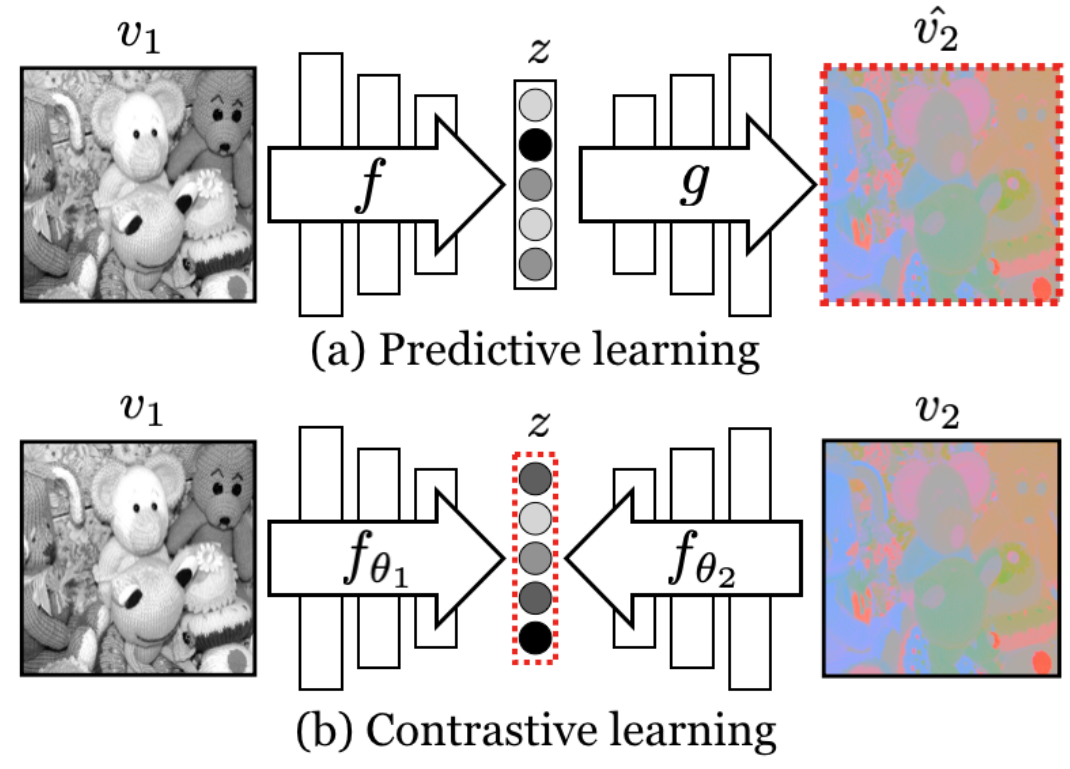
\includegraphics[width=0.9\linewidth]{../../figures/02-04-text-support-img/tian-predictive-vs-contrastive}
        \caption{Predictive Learning vs Contrastive Learning: Contrastive Loss measured in representation space \parencite{tian2020contrastive}}
      \end{figure}
    \end{column}

    \begin{column}{0.5\textwidth}
      \begin{figure}[ht]
        \centering
        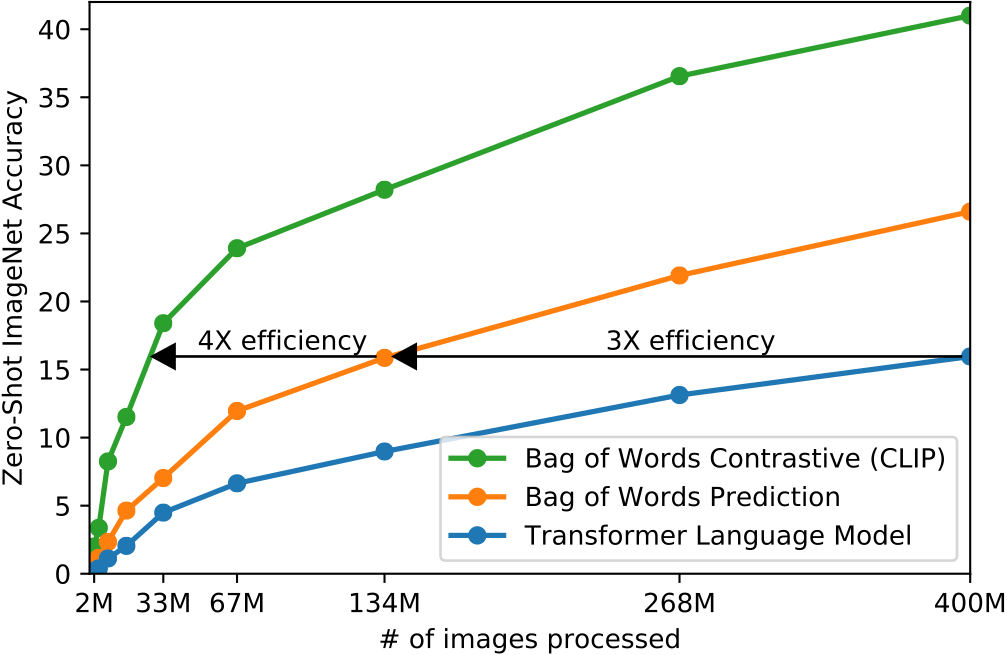
\includegraphics[width=0.9\linewidth]{../../figures/02-04-text-support-img/data-efficiency}
        \caption{Data efficiency of contrastive objective \parencite{radford2021learning}}
      \end{figure}
    \end{column}
  \end{columns}
\end{frame}

\subsection{Zero shooting and foundation models} %------------------------
\begin{frame}{Concepts: Zero shooting and foundation models}
  \begin{itemize}
    \item Paradigms from NLP
    \item Zero shooting: Apply pre-trained model to new, unseen datasets; no deceivement through overfitting
  \end{itemize}

  \begin{figure}[ht]
    \begin{minipage}{0.67\textwidth}
      \centering
      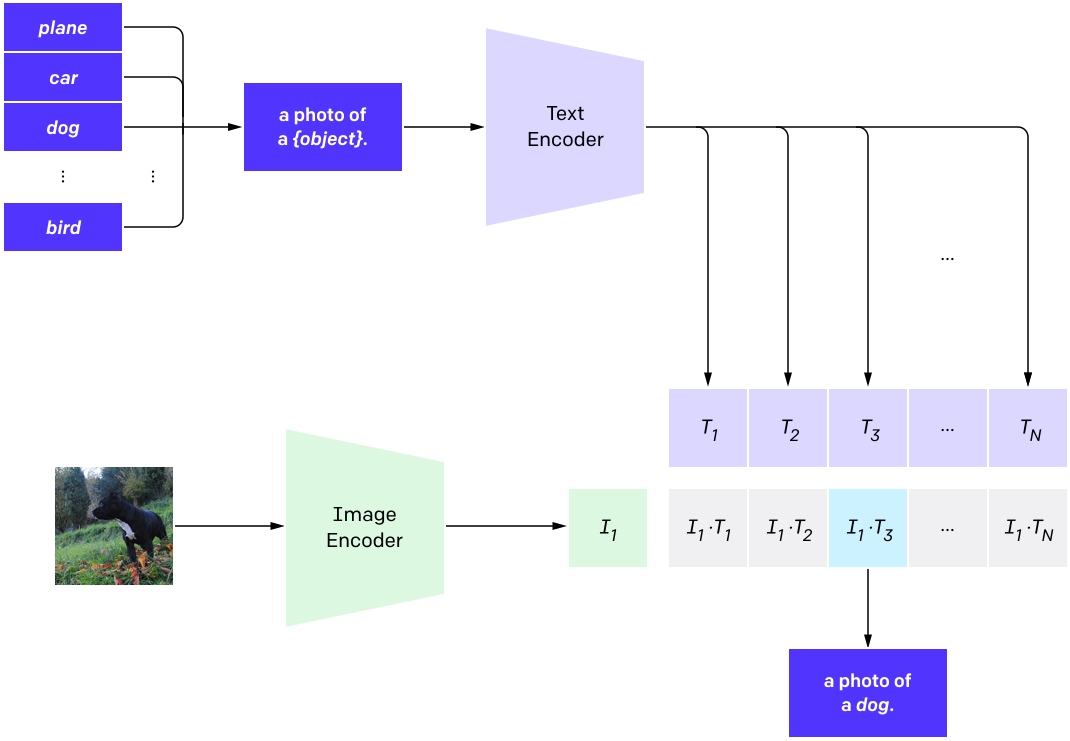
\includegraphics[width=0.8\linewidth]{../../figures/02-04-text-support-img/zero-shooting}
    \end{minipage}
    \begin{minipage}[c]{0.3\textwidth}
      \caption{Visualization of zero-shot application \parencite{radford2021learning}}
    \end{minipage}
  \end{figure}

  \begin{itemize}
    \item Foundation model: Reusing models, e.g., CLIP inside DALL$\cdot$E 2 to embed images \parencite{ramesh2022hierarchical} or as a filter for creating LAION-400M \parencite{schuhmann2022laion}
  \end{itemize}
\end{frame}

\subsection{Connecting image representations to language}
\begin{frame}{Concepts: Connecting image representations to language}
  \begin{itemize}
    \item Learned image representations are directly connected to natural language representations
    \item Direct specification of visual concepts possible through prompt engineering, e.g., \enquote{picture of ...}, \enquote{macro of ...} or \enquote{drawing of ...}
  \end{itemize}
\end{frame}

\section{Architectures} %-------------------------------------------------
\begin{frame}{Contents}
  \tableofcontents[sections={1-3}, currentsection]
  \tableofcontents[sections={4-6}]
\end{frame}


\subsection{CLIP} %-------------------------------------------------------
\begin{frame}{CLIP \parencite{radford2021learning}: Architecture}
  \begin{itemize}
    \item Jointly trained image encoder and text encoder from scratch
    \item Image encoder: Some versions with modified ResNets, some versions with Vision Transformers \parencite[ViT;][]{ImageT}
    \begin{itemize}
      \item ResNet-50, ResNet-101, 3 which follow EfficientNet-style model scaling RN50x4, RN50x16, RN50x64
      \item Vision Transformers: ViT-B/32, ViT-B/16, ViT-L/14, \textbf{ViT-L/14@336px}
    \end{itemize}
    \item Text encoder: Transformer with modifications
    \item Maximization of cosine similarity of image embedding and text embedding
  \end{itemize}
\end{frame}

\begin{frame}{CLIP: Loss}
  Recap: general formulation of contrastive loss

  \begin{equation}
    \ell_1^{V1, V2} = - \underset{\{v_1^1, v_2^1, \ldots, v_2^N\}}{\mathbb{E}} \left( \log \frac{h_\theta(\{v_1^1,v_2^1\})}{h_\theta(\{v_1^1,v_2^1\}) + \sum_{k=2}^N h_\theta(\{v_1^1, v_2^k\})} \right)
  \end{equation}

  Application in CLIP:
  \begin{equation}
    \ell_i^{v_1 \rightarrow v_2} = - \log \frac{\exp(\langle v_1^i, v_2^i \rangle / \tau)}{\sum_{k=1}^{N} \exp(\langle v_1^i, v_2^k \rangle / \tau)},
  \end{equation}

  % \begin{equation}
  %   \ell_i^{v_2 \rightarrow v_1} = - \log \frac{\exp(\langle v_2^i, v_1^i \rangle) / \tau}{\sum_{k=1}^{N} \exp(\langle v_2^i, v_1^k \rangle) / \tau},
  % \end{equation}

  where $\langle v_1^i, v_2^i \rangle$ represents the cosine similarity, i.e., $v_1^{i \top} v_2^i / \|v_1^i\| \|v_2^i\|$; and $\tau \in \mathbb{R}^+$ represents a temperature parameter, which is directly learned during training \parencite{zhang2020contrastive}.
  This can be viewed as a symmetric cross entropy loss over the cosine similarity of the embeddings \parencite{radford2021learning}.
\end{frame}

\begin{frame}{CLIP: Performance}
  \begin{figure}[ht]
    \centering
    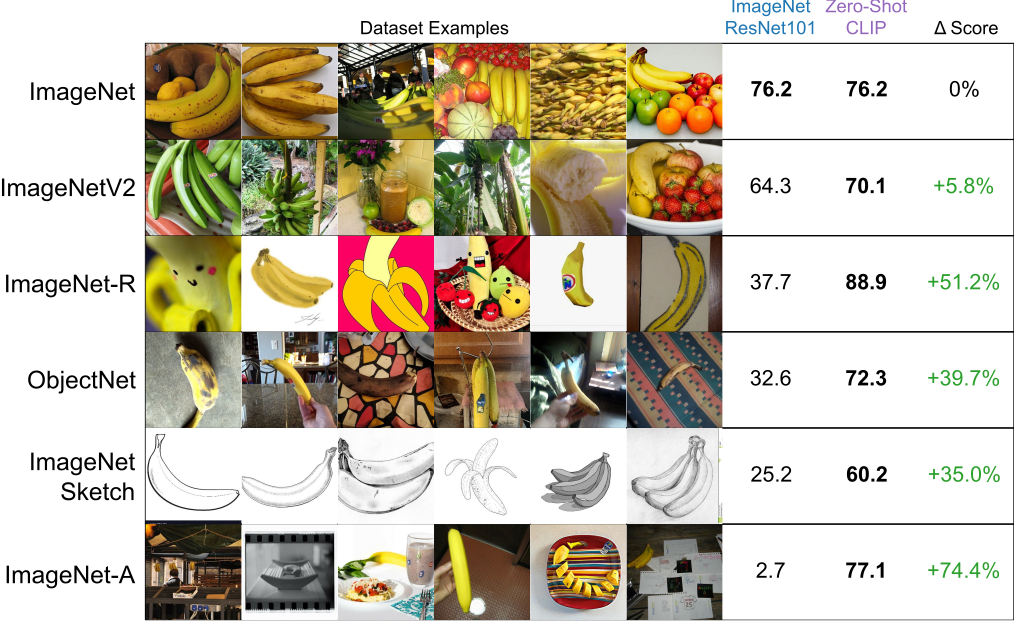
\includegraphics[width=0.7\linewidth]{../../figures/02-04-text-support-img/performance-clip}
    \caption{Robustness of zero-shot CLIP to distribution shifts \parencite{radford2021learning}}
  \end{figure}
\end{frame}

\subsection{ALIGN} %------------------------------------------------------
\begin{frame}{ALIGN \parencite{jia2021scaling}}
  \begin{itemize}
    \item Key difference to CLIP: Less (costly) data curation (400 million image-text pairs $\rightarrow$ 1.8 billion image-text pairs)
    \item Image encoder: EfficientNet (EfficientNet-L2)
    \item Text encoder: BERT (BERT-Large)  % which is basically a transformer
    \item Trained from scratch
    \item 800 million parameters \parencite{alford2021alignparams}
    \item Name: alignment of visual and language representations trough contrastive loss or. Intuitively, "\textbf{A} \textbf{L}arge-scale \textbf{I}ma\textbf{G}e and \textbf{N}oisy-text embedding"
  \end{itemize}
\end{frame}

\begin{frame}{ALIGN \parencite{jia2021scaling}}
  \begin{figure}[ht]
    \centering
    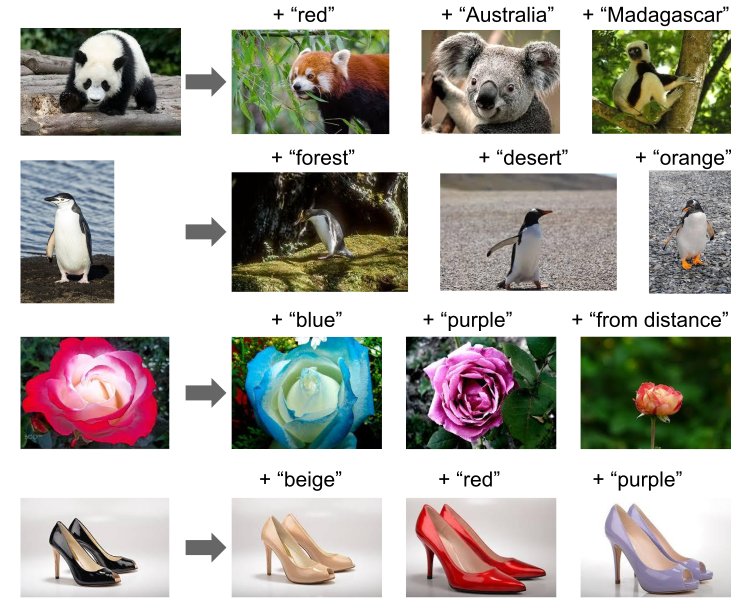
\includegraphics[width=0.7\linewidth]{../../figures/02-04-text-support-img/align-word-and-image-addition}
    \caption{Addition of word and image embedding}
  \end{figure}
\end{frame}

\subsection{Florence} %---------------------------------------------------
\begin{frame}{Florence \parencite{yuan2021florence}}
  \begin{figure}[ht]
    \centering
    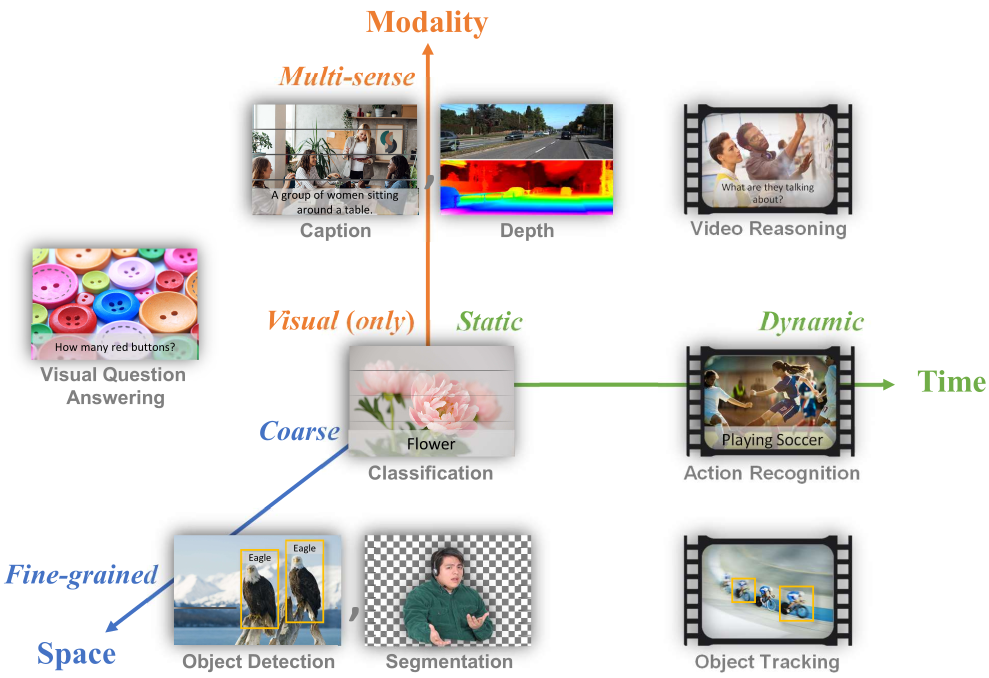
\includegraphics[width=0.7\linewidth]{../../figures/02-04-text-support-img/florence-dimensions}
    \caption{Florence' approach to foundation models: A general purpose vision system for all these tasks.}
  \end{figure}
\end{frame}

\begin{frame}{Florence \parencite{yuan2021florence}}
  \begin{figure}[ht]
    \centering
    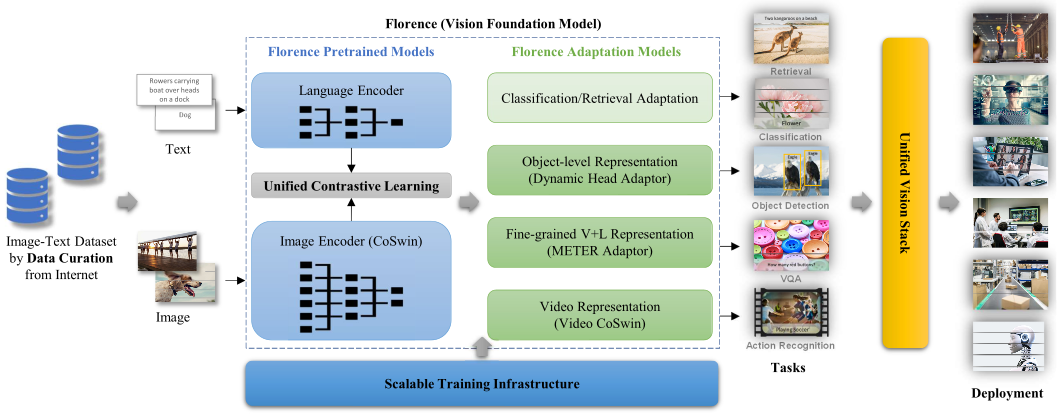
\includegraphics[width=1\linewidth]{../../figures/02-04-text-support-img/florence-architecture}
    \caption{Modular architecture of florence}
  \end{figure}
\end{frame}

\begin{frame}{Florence \parencite{yuan2021florence}}
  \begin{itemize}
    \item Image encoder: hierarchical Vision Transformer (CoSwin Transformer)
    \item Text encoder: Transformer similar to CLIP
    \item Trained from scratch
    \item 893 million parameters \parencite{alford2021alignparams}
    \item 900 million image-text pairs
    \item Name: the origin of the trail for exploring vision foundation models, as well as the birthplace of Renaissance
    \item Loss: unified image-text contrastive learning in image-label-description space $\rightarrow$ All image-text pairs with the same label y are regarded as positive instances.
  \end{itemize}
\end{frame}


\section{Performance comparison} %----------------------------------------
\begin{frame}{Performance comparison}
  \begin{table}[ht]
    \centering
    \resizebox{\textwidth}{!}{
    \begin{tabular}{l|rrrr}
      \hline
               & ImageNet      & ImageNet-R    & ImageNet-A    & ImageNet-V2   \\
      \hline
      CLIP     & 76.2          & 88.9          & \textbf{77.2} & \textbf{70.1} \\
      ALIGN    & 76.4          & \textbf{92.2} & 75.8          & \textbf{70.1} \\
      Florence & \textbf{83.7} &               &               &               \\
      \hline
    \end{tabular}
    }
    \caption{Top-1 Accuracy of zero-shot transfer of ALIGN to image classification on ImageNet and its variants.}
  \end{table}
\end{frame}

\begin{frame}{Performance comparison}
  \begin{table}[ht]
    \centering
    \resizebox{\textwidth}{!}{
    \begin{tabular}{l|rrrr|rrrr}
      \hline
      & \multicolumn{4}{c}{Flickr30K (1K test set)}
      & \multicolumn{4}{|c}{MSCOCO (5K test set)}  \\
      & \multicolumn{2}{c}{Image$\rightarrow$Text}
      & \multicolumn{2}{c}{Text$\rightarrow$Image}
      & \multicolumn{2}{|c}{Image$\rightarrow$Text}
      & \multicolumn{2}{c}{Text$\rightarrow$Image} \\
               & R@1           & R@5           & R@1           & R@5           & R@1           & R@5           & R@1           & R@5           \\
      \hline
      CLIP     & 88.0          & 98.7          & 68.7          & 90.6          & 58.4          & 81.5          & 37.8          & 62.4          \\
      ALIGN    & 88.6          & 98.7          & 75.7          & \textbf{93.8} & 58.6          & 83.0          & 45.6          & 69.8          \\
      Florence & \textbf{90.9} & \textbf{99.1} & \textbf{76.7} & 93.6          & \textbf{64.7} & \textbf{85.9} & \textbf{47.2} & \textbf{71.4} \\
      \hline
    \end{tabular}
    }
    \caption{Zero-shot image and text retrieval \parencite{yuan2021florence}}
  \end{table}
\end{frame}

\begin{frame}{Performance comparison}
  \begin{table}[ht]
    \centering
    \resizebox{\textwidth}{!}{
    \begin{tabular}{l|rrrrrrrrrrrrr}
      \hline
                    & \rot{Food101} & \rot{CIFAR10} & \rot{CIFAR100} & \rot{SUN397} & \rot{Stanford Cars} & \rot{FGCV Aircraft} & \rot{VOC2007} & \rot{DTD}  & \rot{Oxford Pets} & \rot{Caltech101} & \rot{Flowers102} & \rot{ImageNet} \\
      \hline
CLIP                & 93.8    & 95.7    & 77.5     & 68.4   & 78.8          & 37.2          & 84.3    & 55.7 & 93.5        & 92.8       & 78.3       & 76.2 \\
Florence            & 95.1    & 94.6    & 77.6     & 77.0   & 93.2          & 55.5          & 85.5    & 66.4 & 95.9        & 94.7       & 86.2       & 83.7 \\
CLIP (fine tuned)   & 95.9    & \textbf{97.9}    & \textbf{87.4}     & 82.2   & 91.5          & 71.6          & 89.9    & 83.0 & 95.1        & 96.0       & 99.2       & 85.4 \\
ALIGN (fine tuned)  & 95.9    &         &          &        & \textbf{96.1}          &               &         &      & \textbf{96.2}        &            &            & 88.6 \\
Florence (fine tuned) & \textbf{96.2}    & 97.6    & 87.1     & \textbf{84.2}   & 95.7          & \textbf{83.9}          & \textbf{90.5}    & \textbf{86.0} & 96.4        & \textbf{96.6}       & \textbf{99.7}       & \textbf{90.1} \\
      \hline
    \end{tabular}
    }
    \caption{Top-1 Accuracy of CLIP, Florence and ALIGN on various datasets.}
  \end{table}
\end{frame}

\section{Resources} %-----------------------------------------------------
\begin{frame}{Resources}
  \begin{itemize}
    \item Pre-trained CLIP models on Github: \url{https://github.com/openai/CLIP}
    \item Command line image retrieval: rclip, \url{https://github.com/yurijmikhalevich/rclip}
    \begin{itemize}
      \item Wraps \textit{Vit-B/32 CLIP}
    \end{itemize}
  \item CLIP dataset not available $\rightarrow$ Open dataset LAION-400M \parencite{schuhmann2022laion}
  \item Florence code and model weights are not open source \parencite{solawetz2021florenceopen}
  \end{itemize}
\end{frame}

\section{Sources} %-------------------------------------------------------
\begin{frame}[allowframebreaks]{Sources}
  \printbibliography[heading=bibnumbered, title = Bibliography]
\end{frame}

\end{document} %----------------------------------------------------------
